\documentclass[10pt]{beamer}

\usetheme[progressbar=frametitle,numbering=fraction]{metropolis}
\usepackage{appendixnumberbeamer}

\usepackage{booktabs}
\usepackage[scale=2]{ccicons}

\usepackage{pgfplots}
\usepgfplotslibrary{dateplot}

\usepackage{xspace}
\newcommand{\themename}{\textbf{\textsc{metropolis}}\xspace}

\usepackage{graphicx}

\title{Reusing published content in my thesis}
\subtitle{`Happy ending' stories}
\date{24.08.2017}
\author{Vijay Kartik}
\institute{Noon Talk, EPFL Library}
% \titlegraphic{\hfill
\includegraphics[height=1cm]{images/epfl_logo.pdf}}

\begin{document}

\maketitle

\begin{frame}{Table of contents}
  \setbeamertemplate{section in toc}[sections numbered]
  \tableofcontents[hideallsubsections]
\end{frame}

\section{Reusing content}

\begin{frame}[fragile]{What content?}
  \begin{description}
  \item[Step 1:] Write a paper
  \item[Step 2:] Done. I now have (unpublished) content.
  \end{description}
  \vspace{1in}
Ideally, I would already start thinking about how much `freedom' I have with \emph{my own} content.
\end{frame}

\section{Author's rights}

\begin{frame}[fragile]{(Copy) rights}
  Questions to ask:
  \begin{enumerate}
  \item Can I retain copyright? (Answer: \alert{not always})
  \item Can I provide public access to my paper?
  \item Can I use text/images from my paper in my thesis?
  	\begin{itemize}
  		\item Not to self-plagiarize in another paper!
  	\end{itemize}
  \item Where do I submit?
  \end{enumerate}
  P.S.: Sometimes you do not have a say in which journal to publish in (e.g., supervisor decides for you)
\end{frame}

\begin{frame}{Where do I submit?}
	\begin{figure}
		
\includegraphics[trim={0pt 60pt 0pt 0pt}, clip, width=0.5\columnwidth]{images/xkcdjournal}
	\end{figure}
    \hfill \tiny{Source: https://xkcd.com/1847}
\end{frame}

\begin{frame}{Reusing published content in a presentation}
	\alert{Check first!}
	\begin{figure}
		\frame{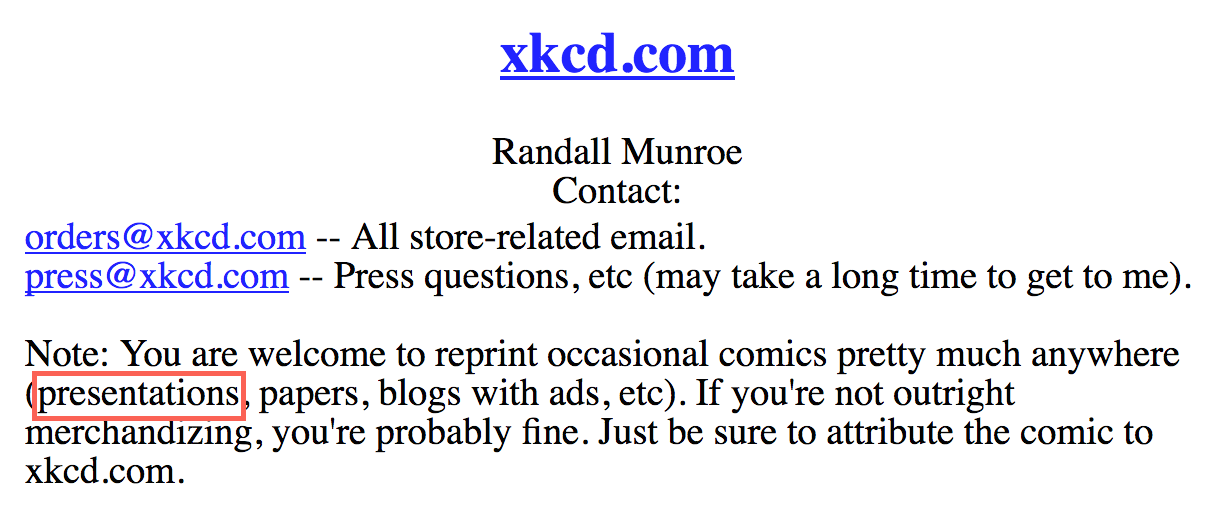
\includegraphics[width=\columnwidth]{images/xkcdpptallowed}}
	\end{figure}
    \hfill \tiny{Source: https://xkcd.com/about}
\end{frame}

\section{\mbox{My experience: pre-emptive confirmations}}

\begin{frame}{Advice: Read \emph{before} signing a licence}
\begin{columns}
\hspace{-60pt}
	\begin{column}{0.6\linewidth}
		\begin{figure}
    		\centering
  			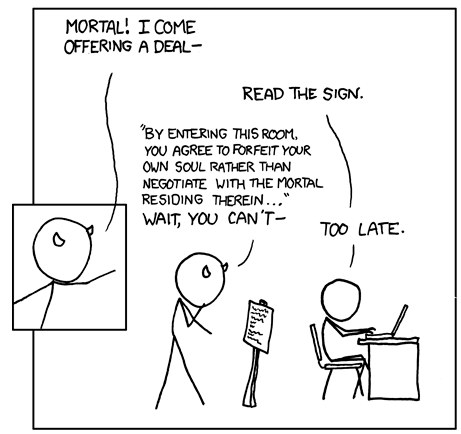
\includegraphics[trim={0pt 0pt 0pt 0pt}, clip, width=\columnwidth]{images/xkcdlicence}
        \end{figure}
        \hfill \tiny{Source: https://xkcd.com/501}
    \end{column}
\hspace{-50pt}
    \begin{column}{0.2\linewidth}
        \begin{figure}
    	    \centering
			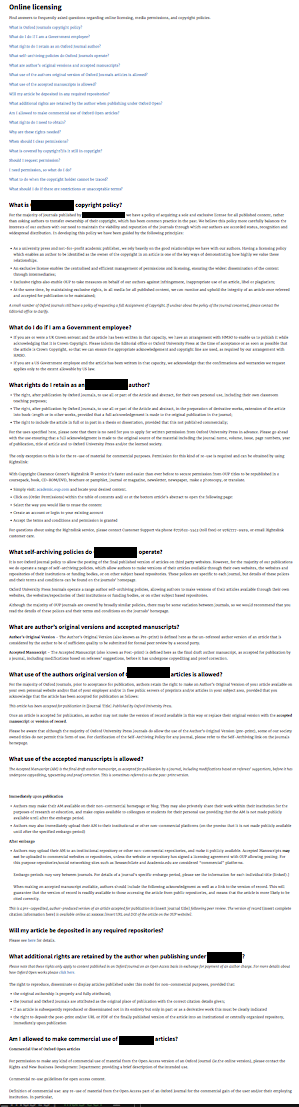
\includegraphics[trim={10pt 0pt 20pt 0pt}, clip, width=\columnwidth]{images/licence}
		\end{figure}
    \end{column}
\end{columns}
\end{frame}

\begin{frame}{Pre/post-prints \& pre/post-embargo}
\begin{columns}
	\begin{column}{0.52\linewidth}
		\begin{figure}
    		\centering
  			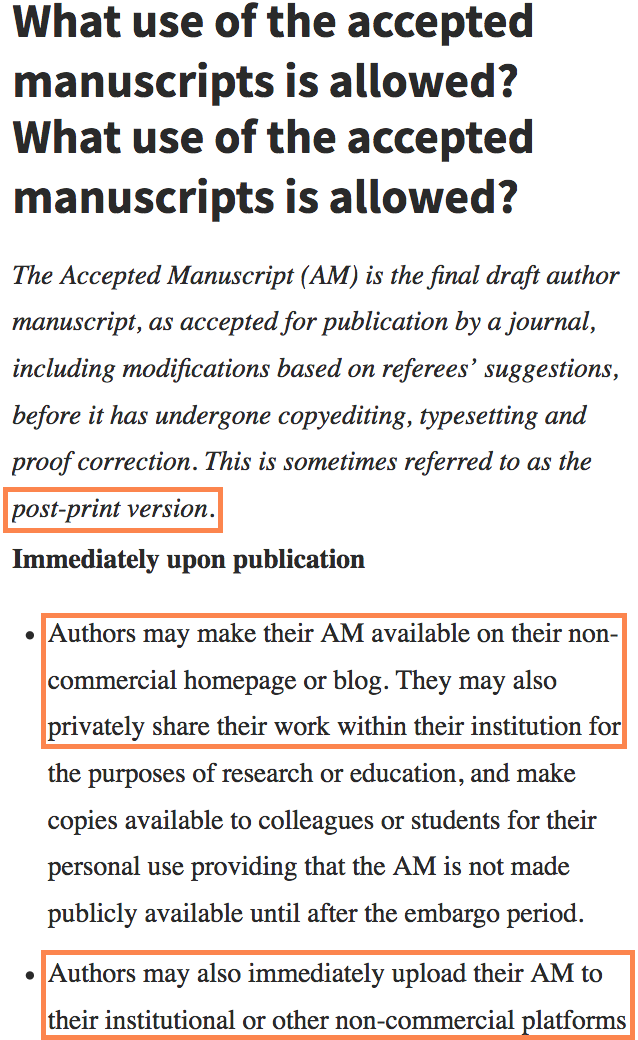
\includegraphics[trim={0pt 0pt 0pt 110pt}, clip, width=\columnwidth]{images/licenceFAQ004a}
        \end{figure}
    \end{column}
    \begin{column}{0.45\linewidth}
        \begin{figure}
    	    \centering
			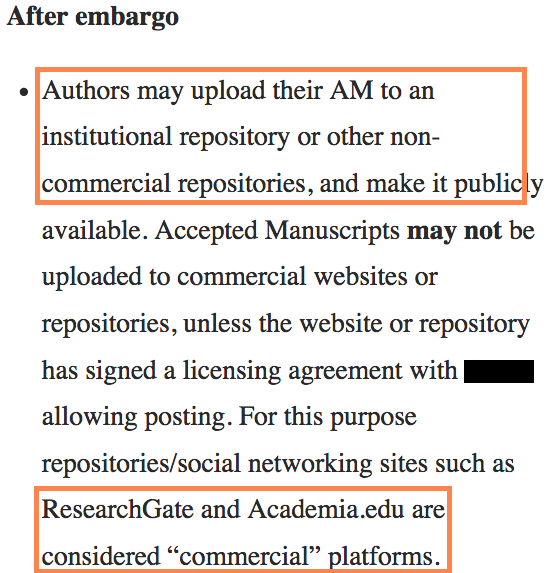
\includegraphics[trim={0pt 0pt 0pt 0pt}, clip, width=\columnwidth]{images/licenceFAQ004b}
		\end{figure}
    \end{column}
\end{columns}
\end{frame}

\begin{frame}{Advice: Look for precise statements}
\hspace{-60pt}
	\begin{figure}
    \centering
		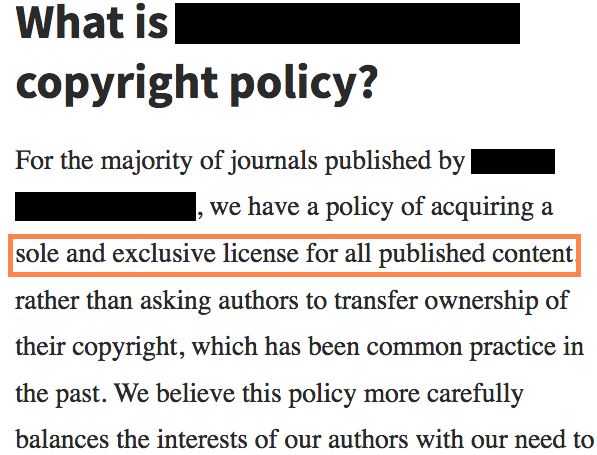
\includegraphics[trim={0pt 0pt 0pt 0pt}, clip, width=\columnwidth]{images/licenceFAQ001}
	\end{figure}
\end{frame}

\begin{frame}{Advice: Check Dos \& Don'ts}
	\begin{figure}
		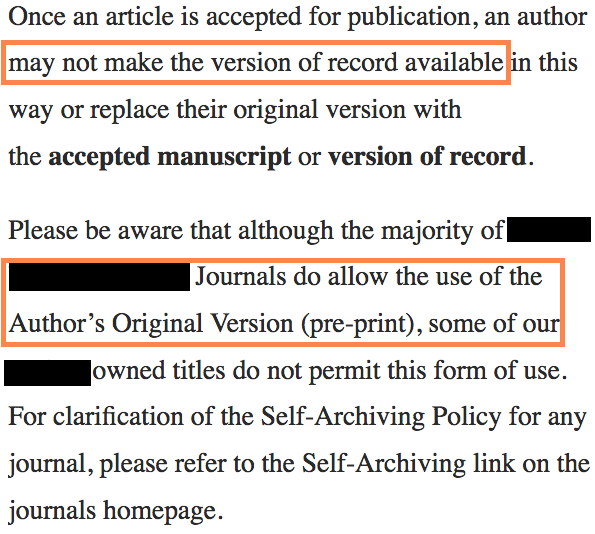
\includegraphics[trim={0pt 30pt 0pt 0pt}, clip, width=\columnwidth]{images/licenceFAQ003}
	\end{figure}
\end{frame}

\begin{frame}{Advice: Ask for \emph{written} clarifications}
	\begin{figure}
		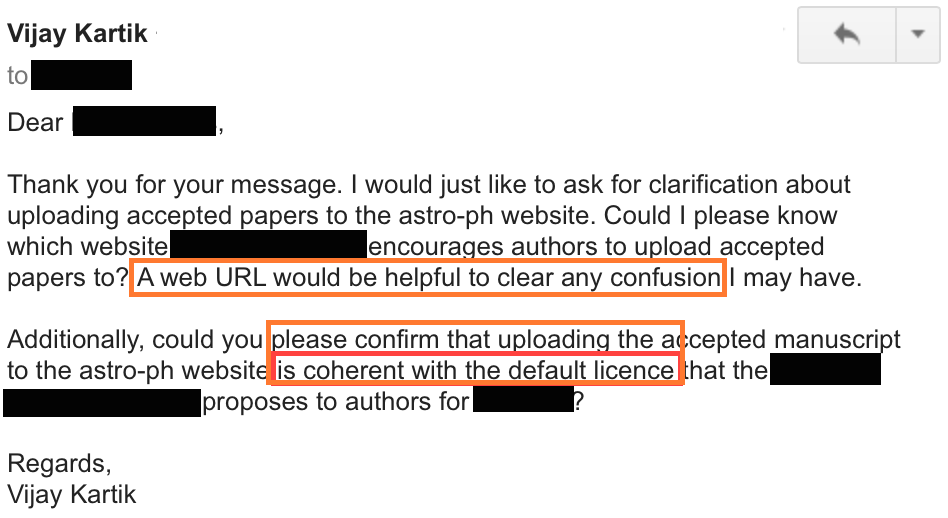
\includegraphics[trim={0pt 0pt 0pt 0pt}, clip, width=0.8\columnwidth]{images/email01}
        
        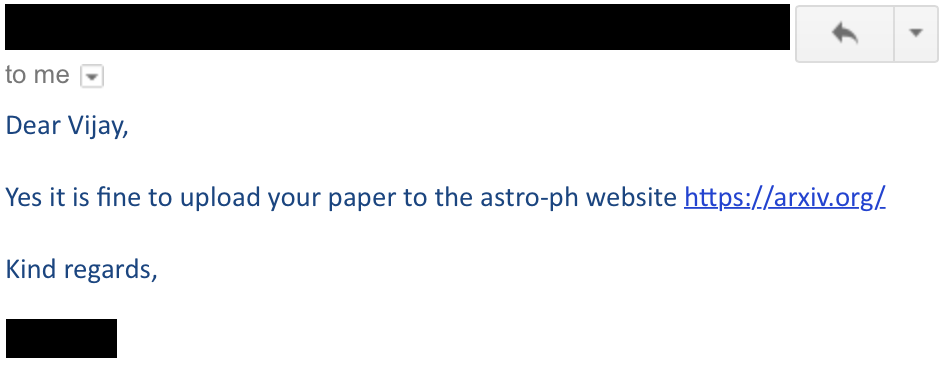
\includegraphics[trim={0pt 0pt 0pt 0pt}, clip, width=0.8\columnwidth]{images/email02}
	\end{figure}
\end{frame}

\begin{frame}{Advice: Seek explicit confirmation}
	\begin{figure}
		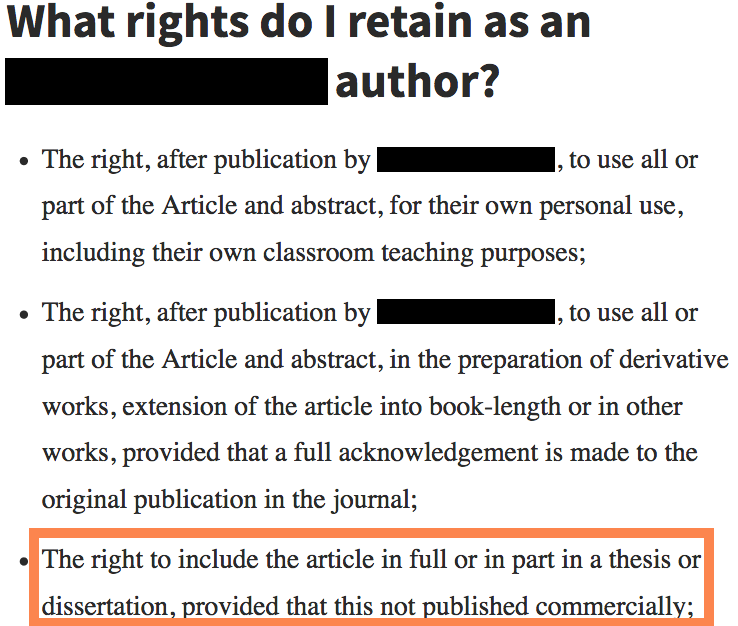
\includegraphics[trim={0pt 0pt 0pt 0pt}, clip, width=0.9\columnwidth]{images/licenceFAQ002}
	\end{figure}
\end{frame}

{\setbeamercolor{palette primary}{fg=black, bg=white}
\begin{frame}[standout, plain, noframenumbering]
  Questions?
\end{frame}
}

\begin{frame}[plain, noframenumbering]{Attributions}
  Get the LaTeX source of this presentation from \textbf{\url{https://github.com/vijaykartik/talk_papersintheses}}
  \vspace{0.5in}
  
  The \themename theme used here is made by Matthias Vogelgesang and licensed under a
  \href{http://creativecommons.org/licenses/by-sa/4.0/}{Creative Commons
  Attribution-ShareAlike 4.0 International License}.
  \begin{center}\ccbysa\end{center}
  \vspace{0.5in}
  
  Screenshots of licensing terms FAQs were taken using public access on publishers' online portals.
\end{frame}

\end{document}
